\section{Kampf starten}\label{sec:kampf-starten}
Nachdem der Nutzer das Starter-Monster erhalten hat, kann er Kämpfe mit anderen (NPC-)Trainern und wilden Monstern starten. Hier ist wichtig zu beachten, dass nur einige NPC-Trainer das Attribut haben, mit dem Nutzer kämpfen zu können.
\subsection{Mockups}\label{subsec:mockups-kampf-starten}
Es gibt mehrere Möglichkeiten zum Start eines Kampfes.
Der Nutzer kann beispielsweise einen anderen Trainer ansprechen und damit einen Kampf mit dem Trainer hervorrufen. Dabei wird im Falle eines NPC-Trainers ein Dialog eröffnet, in dem der NPC-Trainer den Nutzer wie in der Abbildung~\ref{fig: Dialog zwischen Nutzer und NPC-Trainer für Kampf} herausfordert.
Ansonsten wird beim Sprechen mit einem anderen Trainer nur die Ankündigung wie in Abbildung~\ref{fig: Ankündigung über Start des Kampfs} angezeigt, dass der Start des Kampfs in Kürze gestartet wird.
Dabei sieht außerdem der Nutzer den Namen des angesprochenen Trainers.
Darüber hinaus kann ein NPC-Trainer beim Erblicken eines Nutzers versuchen, einen Kampf mit dem Nutzer zu starten. In diesem Fall wird dem Nutzer auch die Ankündigung aus der Abbildung~\ref{fig: Ankündigung über Start des Kampfs} angezeigt.
Beim Drücken der Interaktionstaste gelangt der Nutzer in die Kampfszene wie in Abschnitt~\ref{sec:kampf-führen}.
\begin{figure}[H]
    \center
    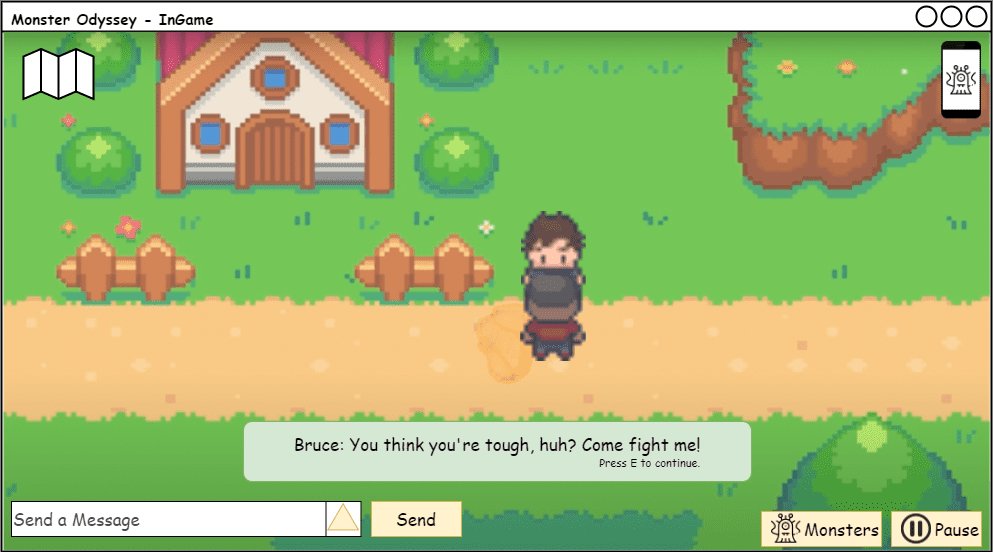
\includegraphics[scale=\scale]{images/mockups/Ingame/PlayerAndNPCStartFight.png}
    \caption{Mockup: Dialog zwischen Nutzer und NPC-Trainer für Kampf}
    \label{fig: Dialog zwischen Nutzer und NPC-Trainer für Kampf}
\end{figure}
\begin{figure}[H]
    \center
    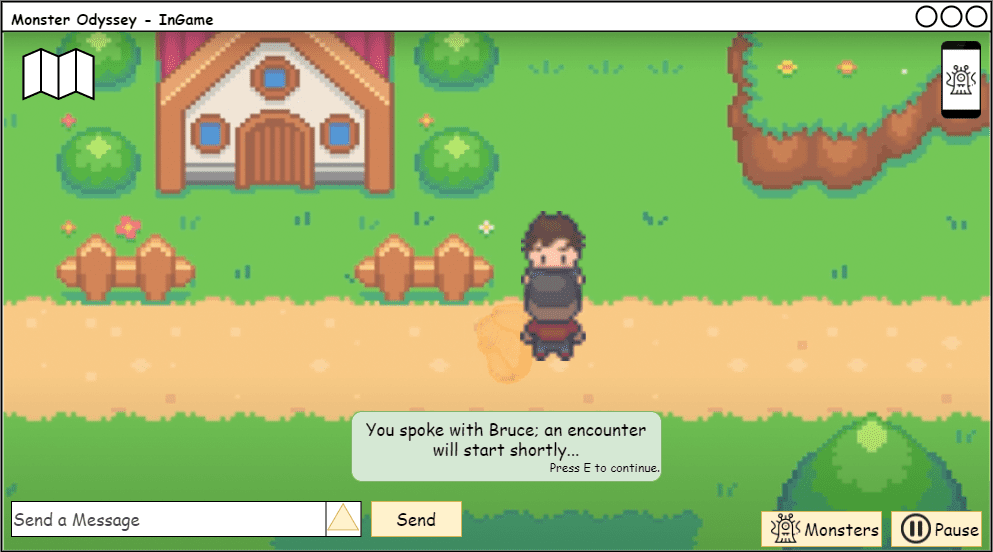
\includegraphics[scale=\scale]{images/mockups/Ingame/PlayerAndPlayerFight.png}
    \caption{Mockup: Ankündigung über Start des Kampfs}
    \label{fig: Ankündigung über Start des Kampfs}
\end{figure}
Außerdem könnte der Nutzer im hohen Gras wilden Monstern begegnen.
Der Kampfstart kommt in diesem Fall nicht von dem Nutzer aus, sondern wird von der Umgebung getroffen.
Um immer noch die Benutzerfreundlichkeit anbieten zu können, wird ebenfalls eine Ankündigung wie in der Abbildung~\ref{fig: Wildem Monster in hohem Gras begegnet} dargestellt.
Gleichermaßen gelangt der Nutzer auch hier beim Drücken der Interaktionstaste in die Kampfszene wie in Abschnitt~\ref{sec:kampf-führen}.
\begin{figure}[H]
    \center
    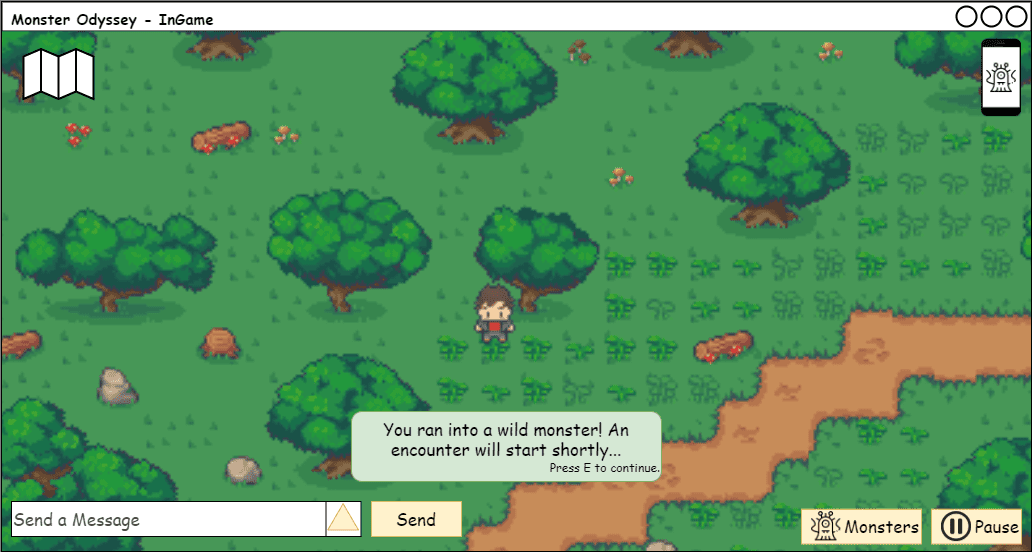
\includegraphics[scale=\scale]{images/mockups/Ingame/PlayerAndWildMonsterFight.png}
    \caption{Mockup: Wildem Monster in hohem Gras begegnet}
    \label{fig: Wildem Monster in hohem Gras begegnet}
\end{figure}
\subsection{Vergleich zwischen Mockups und Implementierung}\label{subsec:vergleich-zwischen-mockups-und-implementierung-kampf-starten}
Vor dem Kampfstart ist in der Implementierung die Ankündigung anders gestaltet. Es wird wie in Abbildung~\ref{fig: Implementierung: Ankündigung über Kampfstart} ein Dialog vor dem Kampfstart geführt, in dem der Sprechende 'Announcement' für die Ankündigung zuständig ist und der Dialogtext wie in der Abbildung~\ref{fig: Mockup: Ankündigung über Kampfstart} ohne den Namen des gegnerischen Trainers festgesetzt ist. Analog gilt es für den Kampf gegen ein wildes Monster. Das Implementieren eines Trainernamens gestaltete sich für die Entwickler schwieriger als erwartet, weshalb der Name weggelassen worden ist.

\begin{figure}[H]
    \centering
    \begin{subfigure}[b]{0.4\textwidth}
        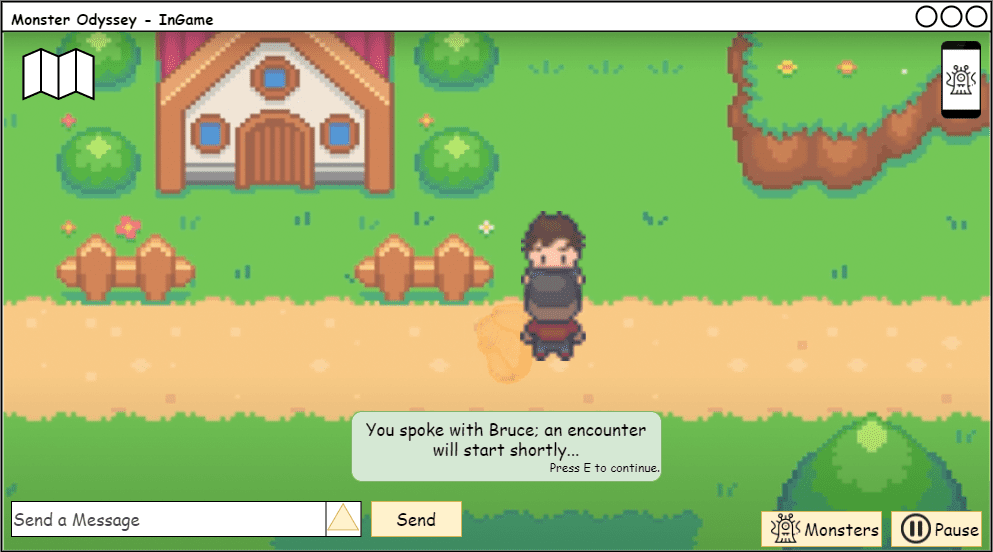
\includegraphics[width=\textwidth]{images/mockups/Ingame/PlayerAndPlayerFight.png}
        \caption{Mockup: Ankündigung über Kampfstart}
        \label{fig: Mockup: Ankündigung über Kampfstart}
    \end{subfigure}
    \hfill
    \begin{subfigure}[b]{0.4\textwidth}
        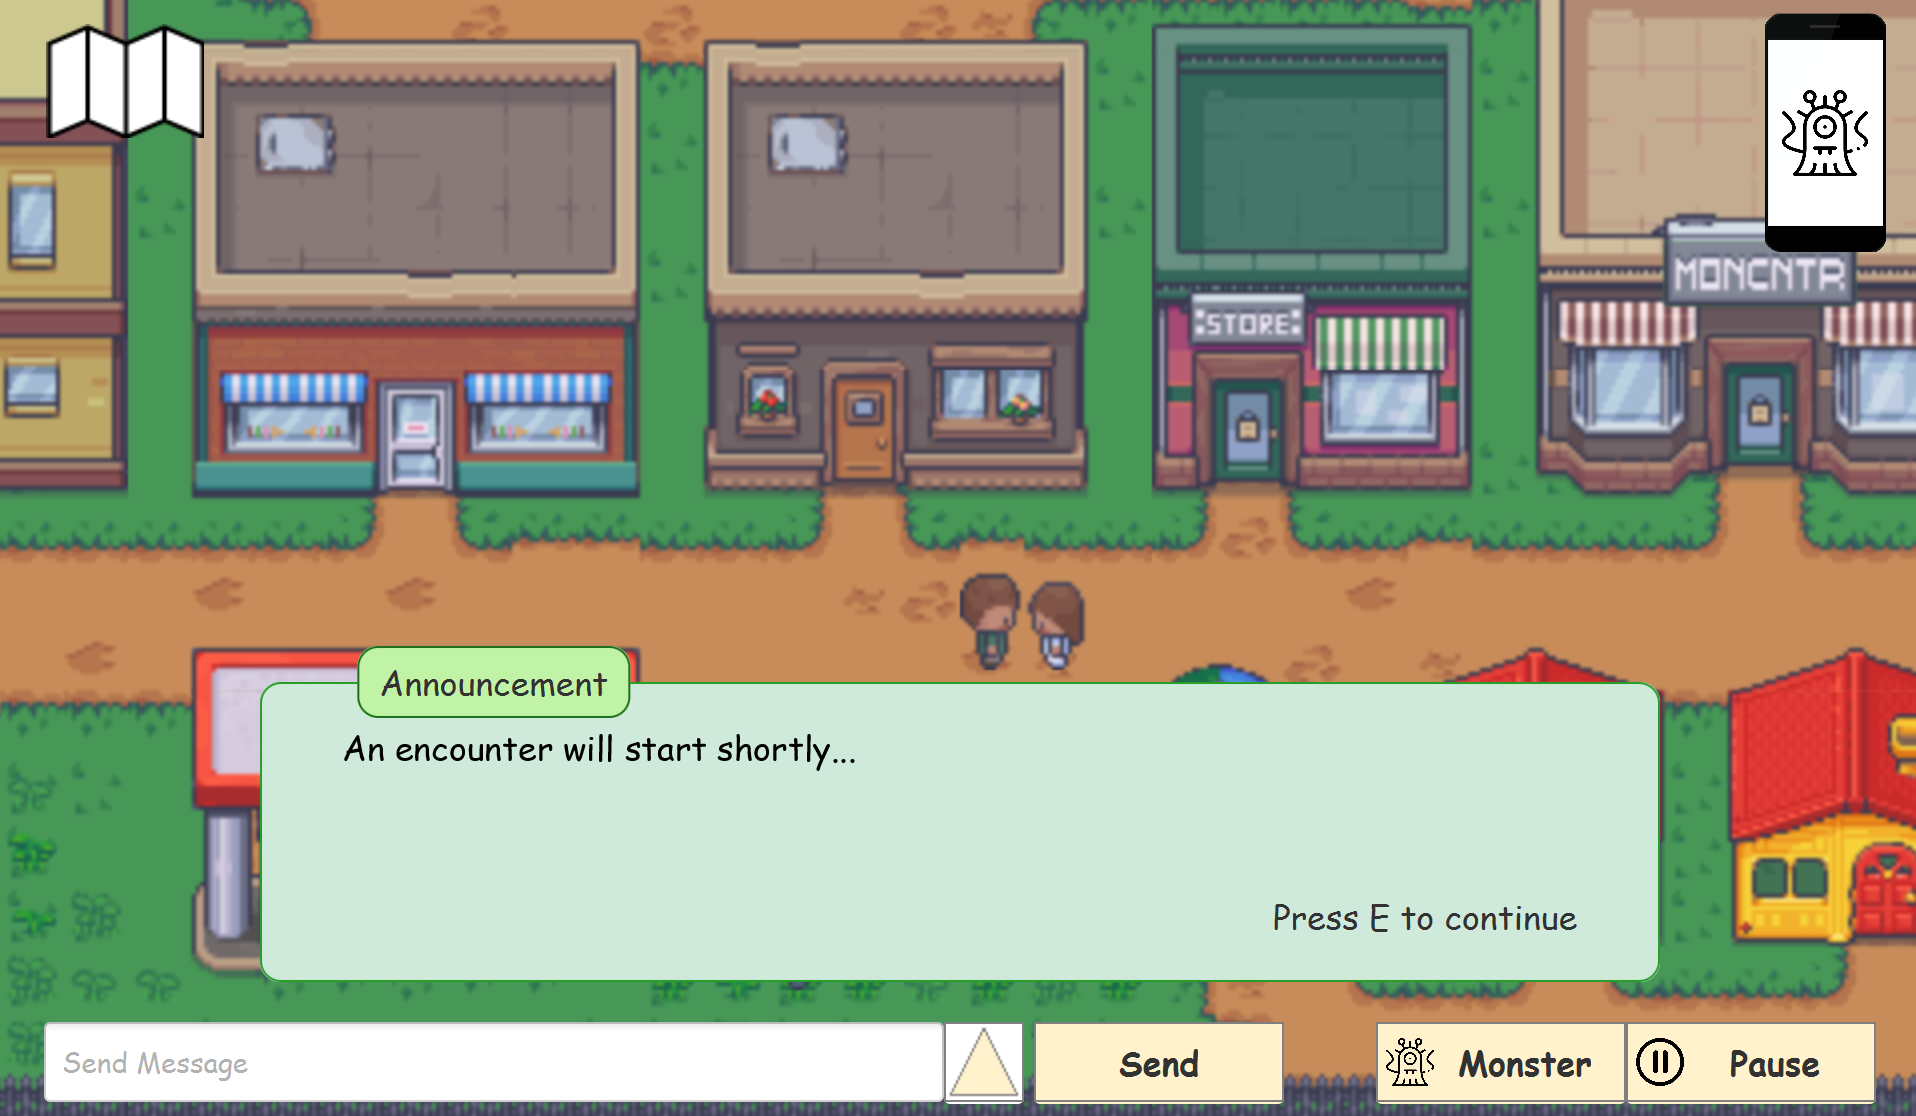
\includegraphics[width=\textwidth]{images/implementation/Ingame/Implementierung anncouncement.png}
        \caption{Implementierung: Ankündigung über Kampfstart}
        \label{fig: Implementierung: Ankündigung über Kampfstart}
    \end{subfigure}
    \caption{Vergleich: Anforderung Kampfstart}
    \label{fig: Vergleich: Anforderung Kampfstart}
\end{figure}